% =============================================================================
\section{The transit viewer and its cache}
\label{sec:transit}
% =============================================================================

\subsection{How it works}

PL7 does not compute the transit animation from scratch each time the time step is
changed. The routines \texttt{CalcMonthEphem} and \texttt{CalcYearEphem}
(\texttt{fcn.0055dc3f}) fill a cache of planetary longitudes, one file per calendar month,
written to \texttt{Temp/YYYYM.e31} (for example \texttt{20201.e31} is January~2020). Two
check boxes in the general options, ``read transit cache'' and ``write transit cache''
(\texttt{general\_readTransitCacheCheckBox}, \texttt{general\_writeTransitCacheCheckBox}),
control whether the files are used \tagBIN. Your installation holds 436 such files covering
January~2020 to April~2056.

The file format was decoded from the data \tagNUM. Bytes 8--23 hold two doubles, the first
and last Julian Day of the month (0h~UT). From byte 840 there is one block of 64 doubles
per body, the block for body $i$ starting at byte $840 + 512\,i$, holding the sidereal
longitude every 12~hours (63 samples for a 31-day month). The body order
Sun, Moon, Mars, Mercury, Jupiter, Venus, Saturn, Rahu was identified from each series'
mean daily motion and position (for example, the first block advances $31.6^\circ$ in
January~2020, the Sun's rate, and the eighth moves retrograde by $0.6^\circ$, a node), and
confirmed by the sub-arcsecond fits below; the later blocks hold slower outer-planet series
and were not used. When you step the viewer forwards or backwards, PL7 interpolates in these
12-hour tables.

\subsection{The cache is not accurate for the planets}
\label{sec:moonvector}

Comparing the cache with the Swiss Ephemeris (Lahiri as in \autoref{eq:lahiri}, mean
equinox) shows two very different behaviours \tagNUM:

\begin{itemize}[leftmargin=*]
  \item \textbf{Moon and Rahu are right.} The Moon agrees after allowing for PL7's larger
  $\Delta T$ (\autoref{sec:deltat}); Rahu agrees to under $1''$.
  \item \textbf{Every other planet is wrong by up to about $10'$,} with an error that
  oscillates once per lunar month (\autoref{fig:moonvector}a).
\end{itemize}

The oscillation has a simple geometric cause. If a planet at geocentric distance $\Delta$
were observed not from the centre of the Earth but from a point displaced by the Moon's
geocentric vector $\vec r_{\text{Moon}}$, its longitude would shift by
\begin{equation}
  \delta\lambda \approx k\,\frac{r_{\text{Moon}}}{\Delta}\,
     \sin(\lambda_{\text{Moon}} - \lambda_{\text{planet}}),
  \label{eq:moonvector}
\end{equation}
with $k = 1$ for the full vector. Regressing each planet's residual on this predictor
explains $R^2 = 0.991$--$0.999$ of the variance, and the fitted coefficient is
$k = 0.967 \pm 0.020$ across 36 planet-months (six planets, six months spread over
2020--2045), independent of the planet's distance (\autoref{fig:moonvector}b) \tagNUM.

\begin{figure}[htbp]
  \centering
  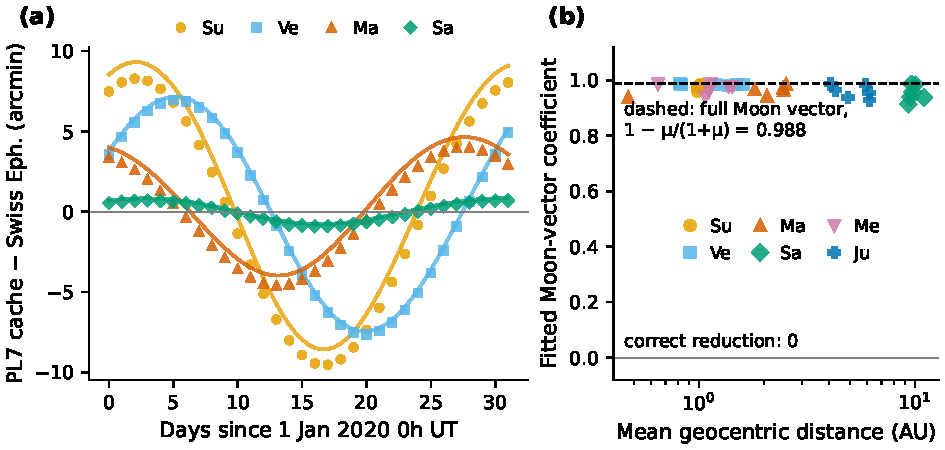
\includegraphics[width=\textwidth]{figures/fig_transit_moon_vector.pdf}
  \caption[The Moon-vector error in PL7's transit cache]{\textbf{PL7's cached planet
  positions are displaced as if seen from a point one Moon-distance away from the Earth.}
  \emph{What is shown.} (a)~Points: PL7's cached sidereal longitude minus the Swiss
  Ephemeris value (monthly mean removed) for the Sun, Venus, Mars and Saturn in January~2020,
  every day; lines: the error predicted by \autoref{eq:moonvector} with
  $k = 1 - \mu/(1+\mu) = 0.988$, no fitting. (b)~The coefficient $k$ fitted separately for
  each of six planets in six months (2020--2045), against the planet's mean geocentric
  distance on a logarithmic axis. The dashed line is the full-Moon-vector prediction; a
  correct Earth--Moon reduction would give $k=0$ (grey line). \emph{What to take from it.}
  The error is not random noise and not a low-precision ephemeris: it is one specific
  geometric mistake whose size shrinks with distance (Sun $\sim\!9'$, Saturn $\sim\!1'$)
  and which the Moon and Rahu escape.}
  \label{fig:moonvector}
\end{figure}

\subsection{Where the error comes from in the code}

Planetary series in such ephemerides are stored for the Earth--Moon barycentre (EMB). To
obtain the Earth, the Moon's geocentric vector is multiplied by $\mu/(1+\mu)$, where
$\mu = M_{\text{Moon}}/M_\oplus \approx 1/81.30$, and subtracted from the EMB. In PL7 this
reduction is in \texttt{fcn.0055e125} \tagBIN. It loads $\mu = 0.01230002$ (address
\texttt{0x5f2e28}) but does \emph{not} divide by the constant $1 + \mu$. Instead it builds
an integer $N$ at run time from four fields of the global application object (offsets
\texttt{0x91c}, \texttt{0x948}, \texttt{0x9b4}, \texttt{0x928}) and uses $\mu/(N + \mu)$:
\begin{equation}
  \text{factor} = \frac{\mu}{N + \mu} =
  \begin{cases} 0.01215 & N = 1 \text{ (correct)},\\ 1 & N = 0. \end{cases}
\end{equation}
With $N = 0$ the whole Moon vector is removed and the planets are seen from a point about
$384\,000$~km from the Earth, consistent with the measured $k = 0.967 \pm 0.020$ (theory
$0.988$). Both planet routines (all-bodies \texttt{fcn.0055ec16} and single-body
\texttt{fcn.0055e5a6}) call this reduction, and both are reached from the one dispatcher
(\texttt{fcn.0055fc12}) used for chart calculation \tagBIN.

The four fields are written mainly inside a block of about ten near-identical code
fragments (\texttt{0x583c7a}--\texttt{0x587xxx}). The PL7 \texttt{readme.txt} says that
the program shipped with a HASP hardware key. A run-time integer that should equal~1 and
silently corrupts results when it does not is a known design for licence-dependent
integrity checks. The installation analysed here was set up following instructions that
replace \texttt{PL7.exe} (\texttt{Important.png} in the \texttt{GeoVision} folder). The most
likely explanation is therefore that this copy runs without the conditions the program
expects, and computes $N = 0$ \tagINF. I did not analyse the licensing code, and the
report gives no instructions about it.

\begin{warnbox}\kpit Because the natal chart uses the same routines, the natal Sun,
Mercury, Venus, Mars, Jupiter and Saturn in \emph{this} installation are probably wrong by
up to about $10'$ as well, while the Moon, Rahu and Ketu, the ascendant and the cusps, and
therefore the Vimshottari dasha, are unaffected. This was \emph{not} directly measured,
because the saved charts (\texttt{GeoVisionCharts/*.xml}) contain only birth data. A
two-minute test is given in \autoref{sec:tests}.\end{warnbox}

\begin{qbox}\kq \emph{``Does this explain why the dasha dates matched Kala Chakra 40/40
while I distrusted the transits?''} Yes. The dasha depends only on the Moon, which this
error does not touch; the transit animation shows the planets, which it does.\end{qbox}
